\documentclass{article}
\usepackage[utf8]{inputenc}
\usepackage{amsmath}
\usepackage{amsfonts}
\usepackage{amssymb}
\usepackage{graphicx}
\usepackage{listings}
\usepackage{xcolor}
\usepackage{minted}
\usepackage{biblatex}
\addbibresource{references.bib}

\title{Understanding Copulas: An Intuitive Guide}
\author{Max Lang}
\date{}

\begin{document}
\maketitle
\begin{figure}
    \centering
    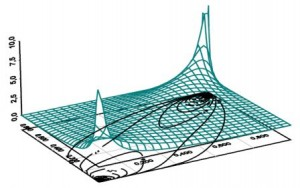
\includegraphics[width=0.75\linewidth]{overviews//copulas//figures/copula.jpg}

\end{figure}
\section{Introduction to Copulas}
Copulas are mathematical tools used in statistics to model and understand the relationship between multiple variables. Their main power lies in separating the marginal distribution of individual variables from their dependence structure. This separation allows researchers to model the dependence structure of variables independently from their margins.

\subsection{Why Use Copulas?}
Copulas are particularly useful in fields like finance and insurance where understanding the correlation between various factors is crucial. They allow for modeling complex dependencies beyond linear correlation, capturing tail dependencies, and more.

\section{Basics of Copulas}
\subsection{Definition}
Formally, a copula is a multivariate cumulative distribution function (CDF) whose marginal probability distributions are all uniform on the interval [0, 1]. According to Sklar's theorem, for any multivariate joint distribution, there exists a copula that links its marginals to the joint distribution function. Mathematically, if $F$ is a joint CDF of random variables $X_1, ..., X_n$ with marginals $F_1, ..., F_n$, then there exists a copula $C$ such that:
$$
F(x_1, ..., x_n) = C(F_1(x_1), ..., F_n(x_n)).
$$

\subsection{Types of Copulas}
Several types of copulas are commonly used, each with its properties and applications:
\begin{itemize}
    \item \textbf{Gaussian Copula:} Uses the correlation matrix of the Gaussian distribution to model dependencies.
    \item \textbf{t-Copula:} Similar to the Gaussian but with heavier tails, capturing tail dependence.
    \item \textbf{Archimedean Copulas:} Include Clayton, Frank, and Gumbel copulas, each modeling different types of dependence structures.
\end{itemize}
\subsection{Sklar's Theorem}
Sklar's Theorem is a cornerstone of copula theory, providing a fundamental link between joint distribution functions and their marginals through copulas. It formalizes the idea that any multivariate distribution can be decomposed into its marginals and a copula that encapsulates the dependency structure among the variables.

\textbf{Theorem (Sklar's Theorem):} Let $F$ be an $n$-dimensional cumulative distribution function (CDF) with marginals $F_1, ..., F_n$. Then there exists a copula $C$ such that for all $x_1, ..., x_n$ in the extended real line,
$$
F(x_1, ..., x_n) = C(F_1(x_1), ..., F_n(x_n)).
$$
Furthermore, if the marginals $F_1, ..., F_n$ are continuous, then $C$ is unique. Conversely, for any copula $C$ and collection of marginals $F_1, ..., F_n$, the function $F$ defined by the above equation is a multivariate CDF with marginals $F_1, ..., F_n$.

\textbf{Implications:} Sklar's Theorem implies that the copula $C$ captures all information about the dependency structure between the variables, independent of their marginal distributions. This separation of dependencies from marginals is what makes copulas a powerful tool in multivariate analysis, allowing for the flexible modeling of complex dependency structures.

\subsection{Applications of Sklar's Theorem}
Sklar's Theorem is not just of theoretical interest; it has practical applications in various fields, including finance, insurance, and risk management. By using copulas, analysts can model dependencies between financial assets, insurance claims, or risks in a way that is independent of the marginal behaviors of these variables. This independence facilitates more accurate modeling of extreme events, tail dependencies, and scenarios where linear correlations fall short.

\subsubsection{Key Properties Derived from Sklar's Theorem}
\begin{enumerate}
    \item \textbf{Decomposition:} Sklar's Theorem allows for the decomposition of a joint distribution into its marginals and a copula, enabling separate modeling of marginal behavior and dependencies.
    \item \textbf{Flexibility:} It provides flexibility in choosing marginals suited to individual variables while using a copula that best describes their joint behavior.
    \item \textbf{Tail Dependency:} Copulas, particularly those beyond the Gaussian copula, can capture tail dependencies (simultaneous extreme values) that are crucial in risk modeling.
\end{enumerate}

Incorporating Sklar's Theorem into the study of copulas enhances the understanding of how copulas function and underscores their value in statistical modeling and analysis.

\section{Intuitive Examples}
To illustrate how copulas work, consider the following examples.

\subsection{Example 1: Financial Asset Returns}
Imagine you want to model the joint distribution of returns on two stocks. You can use historical data to model each stock's margin (e.g., with a normal distribution for each return). Then, use a copula to model the dependence between these returns, capturing aspects like tail dependence, which is crucial for risk management.

\subsection{Example 2: Insurance Claims}
In insurance, copulas can model the dependence between different types of claims. For instance, the likelihood of claims from natural disasters affecting both home and auto insurance. By modeling the margins of each claim type separately and using a copula to model the dependency, insurers can better understand their risk exposure.

\section{Practical Applications}
Copulas are widely used in finance, insurance, hydrology, and other fields where modeling dependencies between variables is essential. They provide a flexible tool for risk management, portfolio optimization, and understanding complex relationships between different factors.

\section{Conclusion}
Copulas offer a powerful and flexible way to model and analyze the dependence between multiple variables, separate from their marginal distributions. By understanding and applying copulas, statisticians and analysts can gain deeper insights into complex, multidimensional relationships.

\printbibliography

\newpage
\appendix
\section{Additional Resources}
For further reading and practical implementations of copulas, refer to the following:
\begin{itemize}
    \item "An Introduction to Copula Theory" by Roger Nelsen
    \item R packages like \texttt{copula} for simulation and analysis.
    \item Python libraries such as \texttt{pycopula} for copula modeling and visualization.
\end{itemize}

\end{document}
